\chapter{Three-dimensional Ultrafast Laser Scanner}
\label{chp:PW2013_Chapter}

Laser scanners are essential for scientific research, manufacturing, defense, and medical practice. Unfortunately, often times the speed of conventional laser scanners (e.g., galvanometric mirrors and acousto-optic deflectors) falls short for many applications, resulting in motion blur and failure to capture fast transient information. Here, we present a novel type of laser scanner that offers roughly three orders of magnitude higher scan rates than conventional methods. Our laser scanner, which we refer to as the hybrid dispersion laser scanner, performs inertia-free laser scanning by dispersing a train of broadband pulses both temporally and spatially. More specifically, each broadband pulse is temporally processed by time stretch dispersive Fourier transform and further dispersed into space by one or more diffractive elements such as prisms and gratings. As a proof-of-principle demonstration, we perform 1D line scans at a record high scan rate of 91 MHz and 2D raster scans and 3D volumetric scans at an unprecedented scan rate of 105 kHz. The method holds promise for a broad range of scientific, industrial, and biomedical applications. To show the utility of our method, we demonstrate imaging, nanometer-resolved surface vibrometry, and high-precision flow cytometry with real-time throughput that conventional laser scanners cannot offer due to their low scan rates.

\section{Introduction}

High-speed multidimensional laser scanning technology has numerous applications in research \cite{marshall2011handbook,fujii2005laser,dotson2003fundamentals,popescu2006optical,gobel2006imaging,pawley2010handbook,denk1990two,wandinger2005lidar}, manufacturing \cite{marshall2011handbook,fujii2005laser,dotson2003fundamentals,schwarz2010mapping,sinha2010vibration,pelesko2002modeling,osten2006optical,horn1986robot}, defense \cite{marshall2011handbook,fujii2005laser,schwarz2010mapping,sinha2010vibration,horn1986robot}, and biomedicine\cite{marshall2011handbook, popescu2006optical,gobel2006imaging,pawley2010handbook,denk1990two,hoffman2006confocal,tarnok2002clinical,vacca2009laser} for sensing and imaging of moving objects and dynamic processes. Low scan rates cause motion blur in images or missing fast transient phenomena in sensing. Also, high-speed scanning capability is needed in high-throughput analysis of a large number of objects or a wide field of view in a reasonable duration of time \cite{marshall2011handbook,fujii2005laser,dotson2003fundamentals,wandinger2005lidar,horn1986robot,hoffman2006confocal,tarnok2002clinical,vacca2009laser,mahjoubfar2011high}.

Various types of laser scanners have been developed over the past few decades. The most commonly used type of laser scanners including MEMS scanners \cite{conant2002micromachined} is based on beam steering by galvanometric mirrors. However, their linear scan rates because of inertia are limited to about 10 kHz. If two of these scanners are aggregated to perform 2-dimensional (2D) raster scans, the overall raster scan rate is limited to about 100 Hz. Another type of laser scanner is based on diverting laser beams by acousto-optic deflectors (AODs). They are about one order of magnitude faster than galvanometric mirror scanners in both linear and 2D raster scans \cite{marshall2011handbook,pape1994design}. Finally, a combination of a frequency-tunable laser and diffractive optics can be used to form a laser scanner at scan rates comparable to AODs \cite{yaqoob2004passive,boudoux2005rapid}.

Recently, we have demonstrated a new type of inertia-free ultra-fast laser scanner that can achieve about three orders of magnitude faster scan rates than the conventional methods \cite{goda2012hybrid}. The operation principle of this method, namely the hybrid dispersion laser scanner (HDLS), is based on probing different points of a target with frequency components of a linearly chirped broadband optical pulse at different times. In this chapter, we present results from our demonstration of linear scans at 90.8 MHz, 2D raster scans at 105.4 kHz, and 3D scanning surface vibrometry with nanometer axial resolution.

\section{Principle of Hybrid dispersion laser scanner}

The concept of HDLS relies on the transformation from spectral to temporal and spatial domains, respectively (Figure \ref{fig:PW2013_Figure1}). First, by a process called dispersive Fourier transformation \cite{kelkar1999time,chou2007femtosecond,goda2009theory,goda2009serial,goda2008amplified} based on group-velocity dispersion, the spectra of broadband optical pulses of a mode-locked laser are mapped into temporal waveforms. Then, a spatial dispersive element such as a diffraction grating or a virtually imaged phased array (VIPA) maps the spectrum of chirped pulses onto a line over the object such that different wavelength components hit the target at different positions and times. The reflected or scattered light from the target is then detected by a single-pixel photodetector. Wavelength components of each laser pulse perform one linear scan, and therefore, the scan rate is same as the repetition rate of the mode-locked laser. A complementary scanner for other axis can be added to achieve 2D raster scans with HDLS.

\begin{figure}[htb!]
\centering
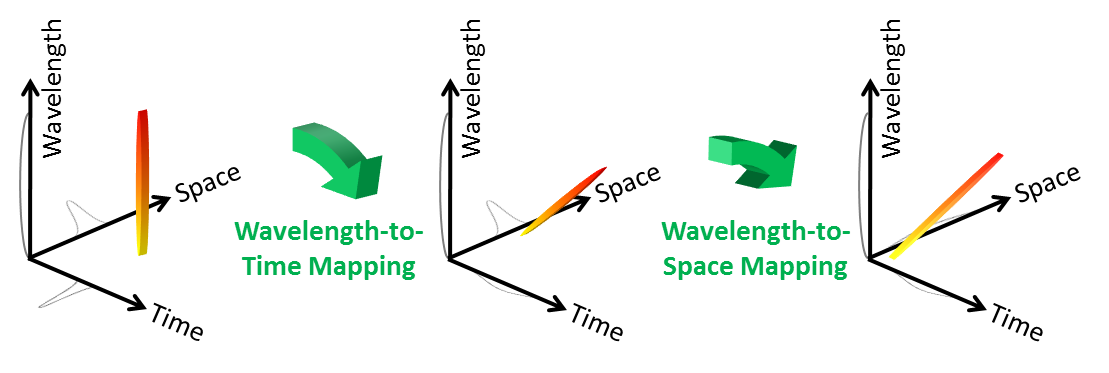
\includegraphics[scale=0.65]{PW2013/Figure1.png}
\caption{Concept of HDLS. HDLS operation relies on two high-speed mapping processes. First, the spectrum of each broadband optical pulse generated by a mode-locked laser is mapped to time. This wavelength-to-time mapping is performed by a temporal dispersive element such as a dispersive optical fiber or prism pair. Next, wavelength-to-space transformation is used to direct each wavelength component of the optical pulse to a unique point on the target. Overall, a one-to-one mapping between time and space is formed. Therefore, each point in HDLS’ field of view is sampled with an individual wavelength component of the optical pulse at a specific time. The repetition rate of the mode-locked laser determines the sampling rate of the HDLS.}
\label{fig:PW2013_Figure1}
\end{figure}

Based on the HDLS concept described, we designed and implemented a multi-dimensional laser scanner in the industrially and biomedically important spectral range of 800 nm (Figure \ref{fig:PW2013_Figure2}). A Ti:Sapphire femtosecond mode-locked laser with a repetition rate of 90.8 MHz generates a train of broadband optical pulses centered at 814 nm. The process of wavelength-to-time mapping is performed with two pairs of prisms followed by a dispersive fiber. Pulses are then collimated into free space and scanned in the vertical direction by an acousto-optic deflector at 105.4 kHz. A pair of diffraction gratings performs the wavelength-to-space mapping, which is the key to fast scanning capability of HDLS at 90.8 MHz in the horizontal direction. 

\begin{figure}[htb!]
\centering
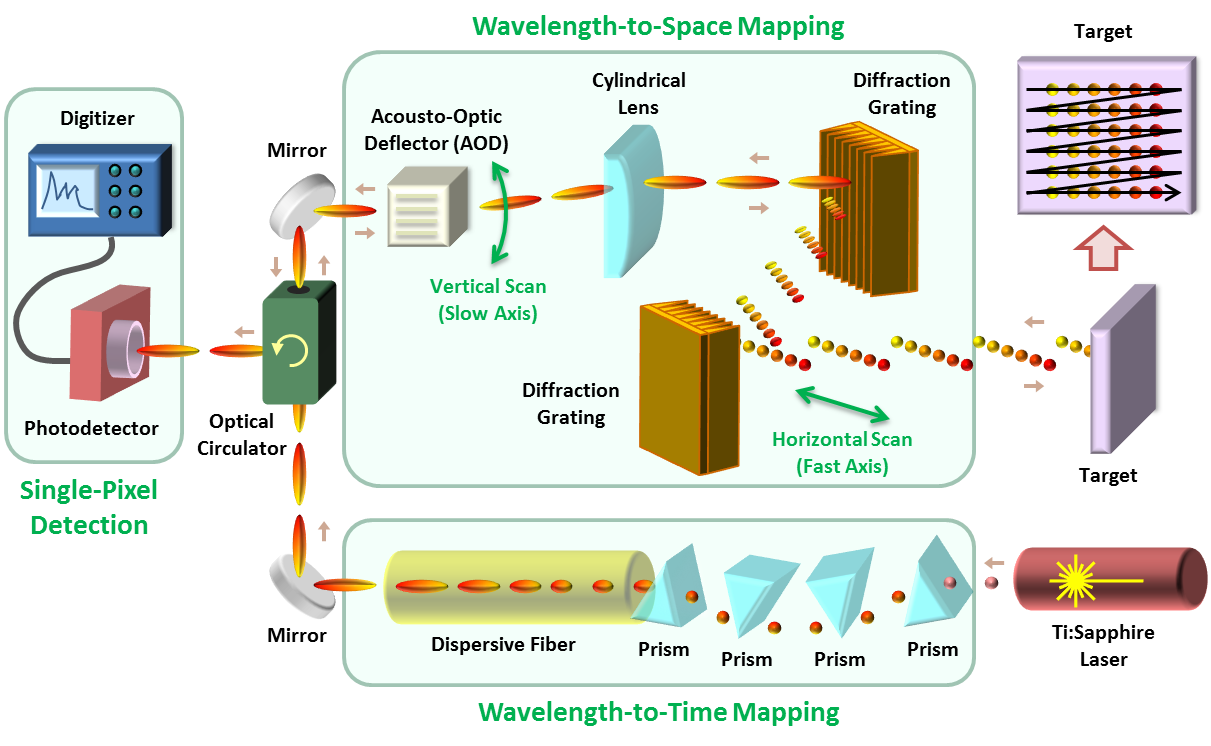
\includegraphics[scale=0.65]{PW2013/Figure2.png}
\caption{HDLS experimental setup. In a 2D demonstration of laser scanning with the HDLS, optical pulses generated by a mode-locked Ti:Sapphire laser with a center wavelength of 814 nm and a repetition rate of 90.8 MHz are dispersed in time using two pairs of prisms and a dispersive fiber. Pulses are deflected in the vertical direction using an acousto-optic deflector (AOD) at 105.4 kHz. Subsequently, the spectrum of each pulse is mapped onto a horizontal line using a pair of diffraction gratings. A combination of the vertical deflection and horizontal mapping leads to a 2D raster scan on the target. The pulse reflection off the surface of the target is converted via an optical circulator to an electrical signal using a single-pixel high-speed photodetector. This is possible due to the prior wavelength-to-time mapping, so that each wavelength component reaches the photodetector at a unique time, and the information of different points of the target are not overlapped. A 50 GS/s digitizer acquires the electrical signal from the photodetector, which corresponds to the spectrum of the optical pulses. After correction for the background envelope, the spectrum of each pulse reveals one horizontal line scan image of the target. Stacking up many of these line scans in accordance with the AOD scan frequency leads to a 2D raster scan of the target.}
\label{fig:PW2013_Figure2}
\end{figure}

Different wavelength components of each laser pulse hit the target at different times, such that a single-pixel photodetector can be used to measure their reflections. The electrical signal of the photodetector corresponding to the waveform of the reflected optical pulses is captured by a high-speed digitizer (50 GS/s, 20 GHz bandwidth oscilloscope) (Figure \ref{fig:PW2013_Figure3}a). Digital waveforms are processed and combined in Matlab to generate multi-dimensional scan profiles. To validate the wavelength-to-time mapping implemented by the prism pairs and dispersive fiber, the spectrum of the reflected pulses from a fixed target is measured with a conventional spectrum analyzer and compared to the waveforms captured by the oscilloscope (Figure \ref{fig:PW2013_Figure3}b). Good agreement between them confirms that we can measure the spectral information of laser pulses at the pulse repetition rate of the mode-locked laser that is well beyond the scan rate of conventional spectrum analyzers.

\begin{figure}[htb!]
\centering
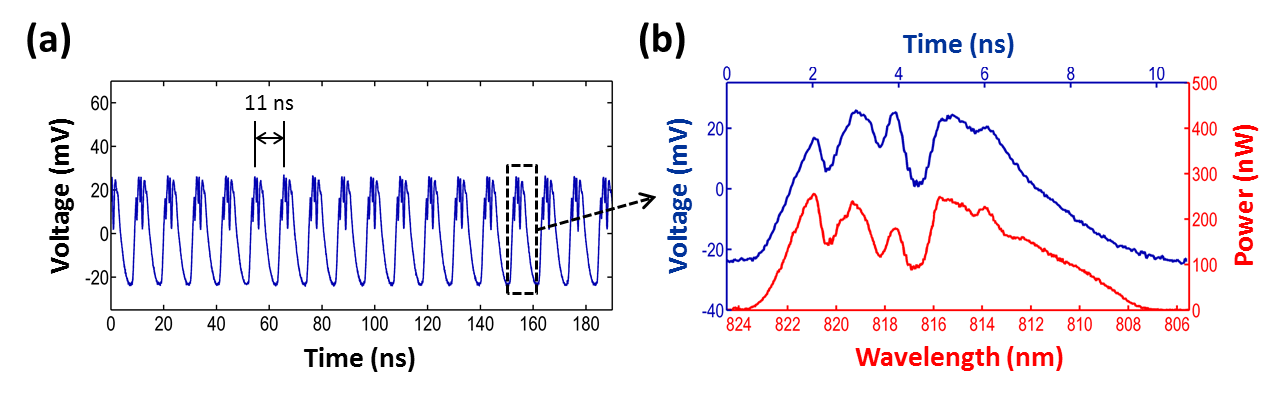
\includegraphics[scale=0.65]{PW2013/Figure3.png}
\caption{Wavelength-to-time mapping with dispersive Fourier transformation. (a) Optical pulses reflected off the target corresponding to horizontal line scans at different deflection angles of the AOD are measured by a high-speed photodetector. The period of the horizontal scans is about 11 ns, which corresponds to the mode-locked laser's pulse repetition rate (90.8 MHz). (b) Good agreement between the amplitude of the photodetector signal measured with the digitizer (shown in blue) and the power spectrum measured with a conventional optical spectrum analyzer indicates the demonstration of the wavelength-to-time mapping using the prism pairs and dispersive fiber in the 800 nm band.}
\label{fig:PW2013_Figure3}
\end{figure}

\section{Applications of Hybrid dispersion laser scanner}

In order to visualize the operation of the HDLS, we scanned a high-reflective substrate with letters “UCLA” engraved on it, and compared the results side-by-side with an image taken by a regular CCD camera (Figure \ref{fig:PW2013_Figure4}). For this experiment, the target was 90 degrees rotated around the illumination axis with respect to the images shown, so that the vertical scans in the image are performed by the HDLS while horizontal scans in the image are implemented by the AOD.

\begin{figure}[htb!]
\centering
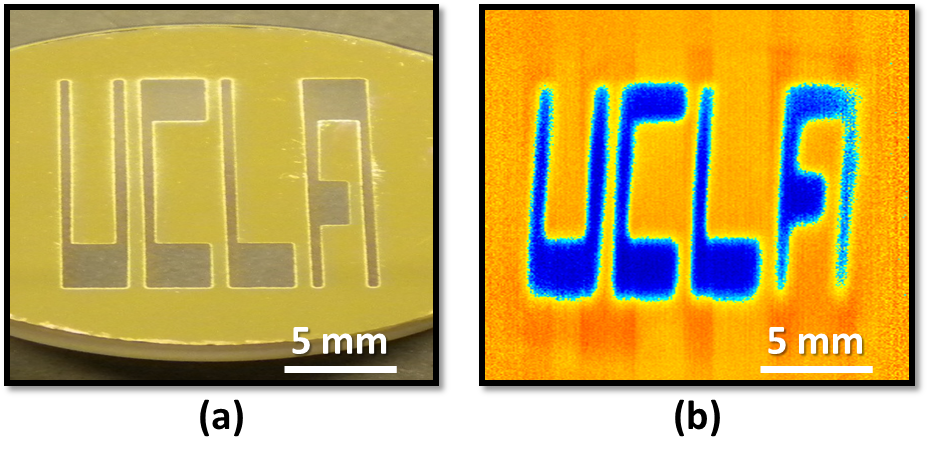
\includegraphics[scale=0.9]{PW2013/Figure4.png}
\caption{Imaging with the HDLS. (a) Image of the word “UCLA” engraved on the surface of a reflective substrate captured by a CCD camera. (b) Image of the same sample captured by the HDLS. The word “UCLA” is clearly shown.}
\label{fig:PW2013_Figure4}
\end{figure}

Combining the HDLS with an interferometer, we performed 3D surface profilometry or 2D surface vibrometry (Figure \ref{fig:PW2013_Figure5}). Here we used a Michelson interferometer to encode phase delays of different points on the target into wavelength components of the illumination pulses. The interferograms are then captured in time, and analyzed offline by Hilbert transformation to extract the phase variations, which correspond to the axial positions. Our experimental setup enables an axial resolution of 0.4 nm at a scan rate of 105.4 kHz. As an illustrative demonstration, we captured vibrations of a reflective diaphragm oscillating at 1 kHz (Figure \ref{fig:PW2013_Figure6}).
 
\begin{figure}[htb!]
\centering
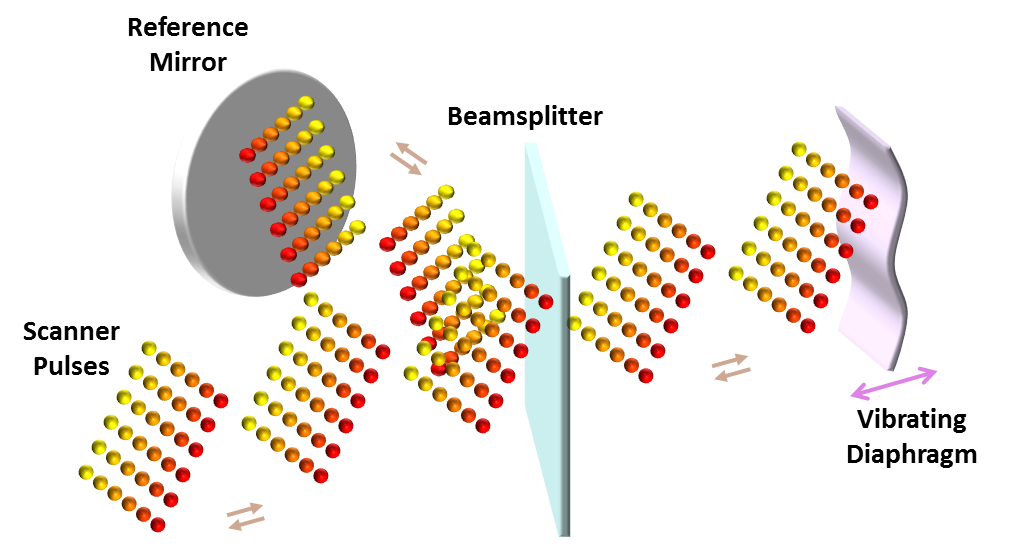
\includegraphics[scale=0.85]{PW2013/Figure5.png}
\caption{3D surface profilometry or 2D surface vibrometry with the HDLS. 2D raster scans by the HDLS are used in conjunction with a Michelson interferometer to perform 2D surface vibrometry. A beamsplitter splits scan pulses into two arms. Optical pulses in one arm hit the target, and the light in the other arm (reference arm) is reflected intactly by a mirror. Reflected pulses from both arms are combined at the beamsplitter and form an interference pattern. If the reflectivity of the vibrating target is not changing rapidly, Hilbert transformation can be used to extract the relative optical phase of each wavelength component. Therefore, variations of the optical path length at each wavelength component are measured and used to form 3D surface profiles of the vibrating sample at a scan rate of 105.4 kHz with 0.4 nanometer axial resolution.}
\label{fig:PW2013_Figure5}
\end{figure}
 
\begin{figure}[htb!]
\centering
\includegraphics[scale=0.68]{PW2013/Figure6.png}
\caption{Surface vibration captured by the HDLS. Frames from 3D scans of a vibrating diaphragm by the HDLS show a period of nanomechanical vibrations at 1 kHz. Only one every ten scan is shown here.}
\label{fig:PW2013_Figure6}
\end{figure}

Finally, as an example of the HDLS’ biomedical utility, we demonstrated high-precision high-throughput flow cytometry using the HDLS. Low spatial resolution of conventional flow cytometers causes a considerable number of false positive events that result in statistical error in subpopulation analysis. For instance, they are not effective for detection of multiple cells (i.e., doublets, triplets, etc.) (Figure \ref{fig:PW2013_Figure7}a). We used inertial focusing microfluidic technology \cite{di2009inertial} to precisely align otherwise randomly positioned cells in a single stream with no need for sheath flow (Figure \ref{fig:PW2013_Figure7}b). The microfluidic channel is custom-made on a substrate dielectric mirror from thermoset polyester (TPE) for stability, robustness, and increased precision of cell focusing. HDLS pulses scan the stream of cells, and the forward scattering is reflected back by the substrate mirror for measurement. 

We tested the performance of the HDLS and conventional flow cytometer for size-based identification of white blood cells and MCF7 breast cancer cells (Figure \ref{fig:PW2013_Figure8}a). Since the HDLS flow cytometer is more precise in distinguishing multiple cells e.g. doublets, the count of white blood cells that have unusually larger size is reduced, and therefore, the false positive rate decreases. This improvement in size-based classification of MCF7 breast cancer cells from white blood cells is more evident in comparison of receiver operating characteristic (ROC) curves of the HDLS and conventional flow cytometer (Figure \ref{fig:PW2013_Figure8}b). We observed that for the same specificity, the sensitivity of our method is significantly higher than that of the conventional flow cytometer. 
 
\begin{figure}[htb!]
\centering
\includegraphics[scale=0.7]{PW2013/Figure7.png}
\caption{Comparison of conventional and HDLS flow cytometers. (a) In regular flow cytometry, a single interrogation beam covers the desired field of view in the channel. Therefore, it does not efficiently differentiate multiple cells such as doublets. In HDLS flow-cytometer, diffraction limited wavelength components of the interrogation beam cover the required field of view, and extract high-resolution spatial information of the sample. HDLS data can be used to identify abnormalities e.g. multiple cells and result in a lower statistical error. (b) In our demonstration of HDLS flow cytometer, an inertial focusing microfluidic channel with a dielectric mirror substrate is used to order randomly distributed cells into a single stream. The microfluidic device was fabricated using standard replica molding methods in thermoset polyester (TPE) to ensure stability. HDLS scan pulses are focused on the stream. Forward-scattered light from the cells is reflected by substrate mirror and collected by an objective lens.}
\label{fig:PW2013_Figure7}
\end{figure}
 
\begin{figure}[htb!]
\centering
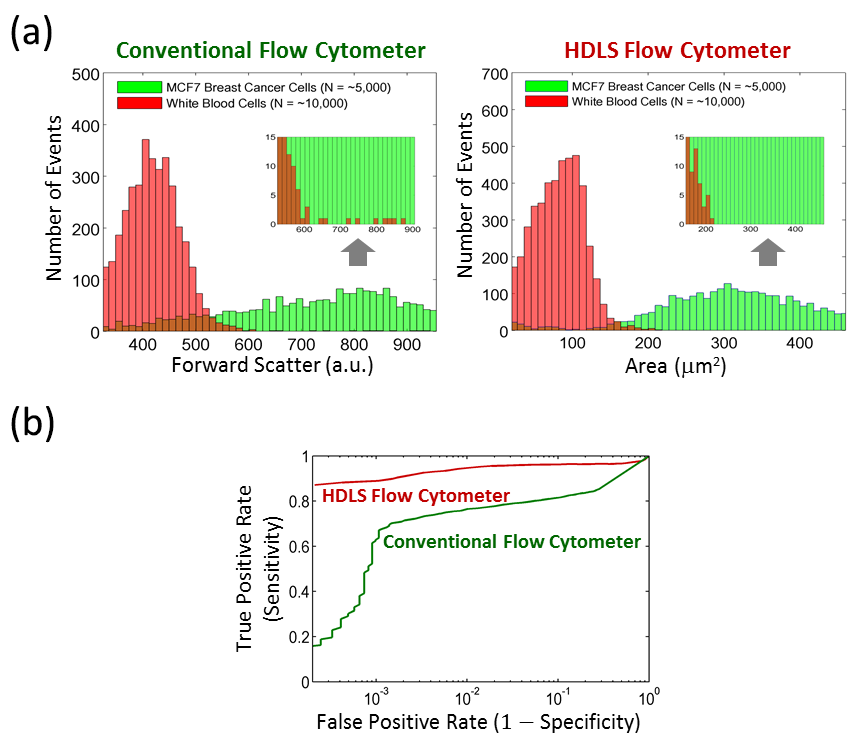
\includegraphics[scale=1]{PW2013/Figure8.png}
\caption{Experimental results of HDLS flow cytometer. (a) Identical samples of white blood cells and MCF7 breast cancer cells are measured separately with conventional and HDLS flow cytometers. There is a considerable overlap in forward scattering range of these cell types for a conventional flow cytometer. However, this overlap decreases significantly for HDLS flow cytometer measurements because white blood cell multiples are not identified as MCF7 cancer cells. (b) Receiver operating characteristic (ROC) curves based on identification of white blood cells and MCF7 breast cancer cells show that without sacrificing throughput, HDLS flow cytometer achieves higher specificity and sensitivity than a conventional flow cytometer.}
\label{fig:PW2013_Figure8}
\end{figure}
